\chapter{Forward and Inverse Simulation}
\label{ch:simulation}

\epigraph{Forward simulation answers ``what happens if\ldots?''\\
Inverse dynamics answers ``what caused this?''}{}

The forward dynamics problem computes accelerations from forces, while inverse dynamics
(also called the inverse kinematics problem when phrased in terms of finding required
torques) computes forces from desired accelerations. Both are fundamental to control design
and trajectory planning.

\section{Forward Dynamics with the Companion Platform}

Forward dynamics integration typically uses explicit or implicit Runge-Kutta methods,
or specialized algorithms such as the Recursive Newton-Euler Algorithm (RNEA) for
rigid-body systems \cite{Featherstone2008, Featherstone1983}.

\begin{lstlisting}[language=Python, caption={Forward dynamics simulation pipeline.}]
import numpy as np
from scipy.integrate import solve_ivp

def forward_dynamics_rnea(
    q: np.ndarray,
    qd: np.ndarray,
    tau: np.ndarray,
    model_params: dict
) -> np.ndarray:
    """Compute joint accelerations using RNEA-based forward dynamics.

    Parameters
    ----------
    q : np.ndarray, shape (n,)
        Joint positions.
    qd : np.ndarray, shape (n,)
        Joint velocities.
    tau : np.ndarray, shape (n,)
        Applied joint torques.
    model_params : dict
        Model parameters (masses, lengths, inertias).

    Returns
    -------
    np.ndarray, shape (n,)
        Joint accelerations.
    """
    n = len(q)
    masses = model_params['masses']
    lengths = model_params['lengths']
    g = model_params.get('gravity', 9.81)

    # Simple 2-link model for demonstration
    if n == 2:
        m1, m2 = masses[:2]
        l1, l2 = lengths[:2]
        lc1, lc2 = l1/2, l2/2
        I1 = m1 * l1**2 / 12
        I2 = m2 * l2**2 / 12

        # Mass matrix
        M = np.array([
            [I1 + I2 + m1*lc1**2 + m2*(l1**2 + lc2**2 + 2*l1*lc2*np.cos(q[1])),
             I2 + m2*(lc2**2 + l1*lc2*np.cos(q[1]))],
            [I2 + m2*(lc2**2 + l1*lc2*np.cos(q[1])),
             I2 + m2*lc2**2]
        ])

        # Coriolis
        h = m2 * l1 * lc2 * np.sin(q[1])
        C = np.array([[-h*qd[1], -h*(qd[0]+qd[1])],
                       [h*qd[0], 0]])

        # Gravity
        gvec = np.array([
            (m1*lc1 + m2*l1)*g*np.sin(q[0]) + m2*lc2*g*np.sin(q[0]+q[1]),
            m2*lc2*g*np.sin(q[0]+q[1])
        ])

        qdd = np.linalg.solve(M, tau - C @ qd - gvec)
    else:
        # Placeholder for general n-DOF
        qdd = np.zeros(n)

    return qdd

# Example simulation
params = {'masses': [2.0, 1.0], 'lengths': [0.3, 0.25], 'gravity': 9.81}
q0 = np.array([np.pi/4, np.pi/6])
qd0 = np.zeros(2)
qdd = forward_dynamics_rnea(q0, qd0, np.zeros(2), params)
print(f"Gravity-driven accelerations: {qdd}")
\end{lstlisting}

\section{Simulation Loop and Integration Schemes}

Figure~\ref{fig:sim-loop} illustrates the typical forward simulation loop. At each
timestep, we compute accelerations from the equations of motion, integrate to update
velocities and positions, and advance to the next timestep.

\begin{figure}[h]
  \centering
  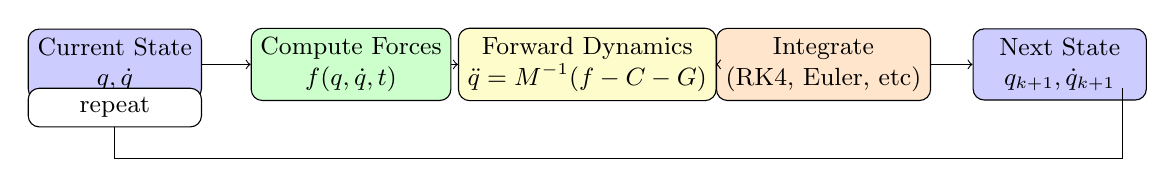
\begin{tikzpicture}[
    every node/.style={align=center, draw, rounded corners, minimum width=2.2cm, text centered, font=\small},
    ]
    % State
    \node[fill=blue!20] (state) at (0, 0) {Current State\\$\bm{q}, \dot{\bm{q}}$};
    % Compute accelerations
    \node[fill=green!20] (forces) at (3, 0) {Compute Forces\\$\bm{f}(\bm{q}, \dot{\bm{q}}, t)$};
    % Solve dynamics
    \node[fill=yellow!20] (dynamics) at (6, 0) {Forward Dynamics\\$\ddot{\bm{q}} = M^{-1}(\bm{f} - C - G)$};
    % Integrate
    \node[fill=orange!20] (integrate) at (9, 0) {Integrate\\(RK4, Euler, etc)};
    % Next state
    \node[fill=blue!20] (next) at (12, 0) {Next State\\$\bm{q}_{k+1}, \dot{\bm{q}}_{k+1}$};

    % Arrows
    \draw[->] (state) -- (forces);
    \draw[->] (forces) -- (dynamics);
    \draw[->] (dynamics) -- (integrate);
    \draw[->] (integrate) -- (next);
    \draw[->] (12.8, -0.3) -- (12.8, -1.2) -- (0, -1.2) -- (0, -0.4) node[align=center, above, pos=0.5, fill=white] {repeat};
  \end{tikzpicture}
  \caption{Forward simulation loop: from current state to forces (gravity, contacts, actuators),
    compute accelerations via forward dynamics, integrate, and update to next state.}
  \label{fig:sim-loop}
\end{figure}

\section{Inverse Dynamics Pipeline}

The inverse dynamics problem solves for torques given desired motion: given $\bm{q}(t),
\dot{\bm{q}}(t), \ddot{\bm{q}}(t)$, compute $\bm{\tau}(t)$. This is implemented via the
Recursive Newton-Euler Algorithm (RNEA) \cite{Featherstone2008, luh1980}. The RNEA
can be run either forward (for forward dynamics) or backward (for inverse dynamics)
through the kinematic chain.

\section*{Exercises}
\begin{enumerate}
  \item Run forward dynamics for a 2-link pendulum and plot trajectories.
  \item Implement inverse dynamics and verify $\text{ID}(\text{FD}(\tau)) = \tau$.
  \item Compare with Pinocchio's RNEA implementation for timing.
\end{enumerate}
